\documentclass{article}
\usepackage{graphicx}
\usepackage{amsmath,amssymb}
\setlength{\parindent}{0pt}
\usepackage{listings}
\usepackage{lmodern}  % for bold teletype font
\usepackage{amsmath}  % for \hookrightarrow
\usepackage{xcolor}   % for \textcolor
\usepackage[a4paper,margin=1in,footskip=0.25in]{geometry}
\usepackage{graphicx}

\lstset{
  basicstyle=\ttfamily,
  columns=fullflexible,
  frame=single,
  breaklines=true,
}

\begin{document}

\title{Deep Reinforcement Learning Project 2 : Continuous Control}
\author{Rachel Schlossman}

\maketitle

\section{Learning Algorithm}
The learning algorithm is an implementation of the Deep Deterministic Policy Gradient algorithm as described in \cite{lillicrap2015continuous}. As the paper describes, the algorithm leverages (1) an actor network to approximate actor function $\mu(s|\theta^{\mu})$ and a critic network to approximate the action-value function, $Q(s,a|\theta^Q)$ using the Bellman Equation (similar to Q-learning). The variable $s$ is the state, $a$ is the action, and $\theta^{\mu}$ and $\theta^{Q}$ are the actor and critic network weights, respectively.  The algorithm is suited only for continuous action spaces.

\subsection{Hyperparameters}
The following hyperparameters were used in the DDPG implementation:

\begin{itemize}
\item replay buffer size : 1e6
\item minibatch size: 128
\item discount factor: 0.99 
\item for soft update of target parameters, $\tau$: 1e-3
\item learning rate of the actor: 1e-4  
\item learning rate of the critic: 1e-4 
\item L2 weight decay: 0
\end{itemize}

It is also important to note that the selection of the maximum number of timesteps in an episode, max\_t, was critical for agent learning. When max\_t originally equaled 300, the average reward plateaued at about 10. After increasing max\_t to 20,000 and maintaining the hyperparameters listed above, the agent reached the desired average reward of +30.

\section{Model Architecture}
The DDPG algorithm employs to neural networks, the actor network and the critic network. Form both networks, the input passes through two linear layers with relu activation. For the actor network, the hidden layers are followed by a tanh output layer. For the critic network, the hidden layers are followed by a linear output layer. The two hidden layers for each network each are comprised of 256 nodes. The code implementation is shown below. 

\begin{lstlisting}[language=Python]
def hidden_init(layer):
    fan_in = layer.weight.data.size()[0]
    lim = 1. / np.sqrt(fan_in)
    return (-lim, lim)

class Actor(nn.Module):
    """Actor (Policy) Model."""

    def __init__(self, state_size, action_size, seed, fc1_units=256, fc2_units=256):
        """Initialize parameters and build model.
        Params
        ======
            state_size (int): Dimension of each state
            action_size (int): Dimension of each action
            seed (int): Random seed
            fc1_units (int): Number of nodes in first hidden layer
            fc2_units (int): Number of nodes in second hidden layer
        """
        super(Actor, self).__init__()
        self.seed = torch.manual_seed(seed)
        self.fc1 = nn.Linear(state_size, fc1_units)
        self.fc2 = nn.Linear(fc1_units, fc2_units)
        self.fc3 = nn.Linear(fc2_units, action_size)
        self.reset_parameters()

    def reset_parameters(self):
        self.fc1.weight.data.uniform_(*hidden_init(self.fc1))
        self.fc2.weight.data.uniform_(*hidden_init(self.fc2))
        self.fc3.weight.data.uniform_(-3e-3, 3e-3)

    def forward(self, state):
        """Build an actor (policy) network that maps states -> actions."""
        x = F.relu(self.fc1(state))
        x = F.relu(self.fc2(x))
        return F.tanh(self.fc3(x))


class Critic(nn.Module):
    """Critic (Value) Model."""

    def __init__(self, state_size, action_size, seed, fcs1_units=256, fc2_units=256):
        """Initialize parameters and build model.
        Params
        ======
            state_size (int): Dimension of each state
            action_size (int): Dimension of each action
            seed (int): Random seed
            fcs1_units (int): Number of nodes in the first hidden layer
            fc2_units (int): Number of nodes in the second hidden layer
        """
        super(Critic, self).__init__()
        self.seed = torch.manual_seed(seed)
        self.fcs1 = nn.Linear(state_size, fcs1_units)
        self.fc2 = nn.Linear(fcs1_units+action_size, fc2_units)
        self.fc3 = nn.Linear(fc2_units, 1)
        self.reset_parameters()

    def reset_parameters(self):
        self.fcs1.weight.data.uniform_(*hidden_init(self.fcs1))
        self.fc2.weight.data.uniform_(*hidden_init(self.fc2))
        self.fc3.weight.data.uniform_(-3e-3, 3e-3)

    def forward(self, state, action):
        """Build a critic (value) network that maps (state, action) pairs -> Q-values."""
        xs = F.relu(self.fcs1(state))
        x = torch.cat((xs, action), dim=1)
        x = F.relu(self.fc2(x))
        return self.fc3(x)

\end{lstlisting}

\section{Results}
The parallel agents are able to receive an average reward (over 100 episodes, and over all 20 agents) of at least +30 in 104 episodes, as shown in Fig. \ref{fig:results}.

\begin{figure}[ht]
\centering
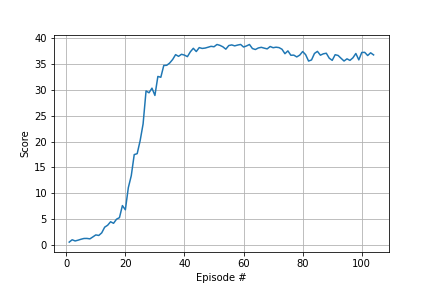
\includegraphics[scale=0.75]{./figures/results.png}
\caption{Average Score Plot}
\label{fig:results}
\end{figure}

\section{Future Work}
The optimal value for the variable max\_t could be explored further so that it could be reduced (thereby decreasing simulation time) while still maintaining the desired level of agent learning. From reviewing OpenAI Spinning Up's implmentation, it could also be useful to reduce the scale of the Ornstein–Uhlenbeck process noise as training advances. Spinning Up also described ``Our DDPG implementation uses a trick to improve exploration at the start of training. For a fixed number of steps at the beginning, the agent takes actions which are sampled from a uniform random distribution over valid actions. After that, it returns to normal DDPG exploration \ref{SpinningUp2018}." This detail could also be interesting future work. 

\bibliographystyle{plain}
\bibliography{bib}

\end{document}